The protein structure is represented by 11 density maps corresponding
to the atom types defined in Table \ref{Tbl:atomTypes}. These atom
types are a simplification of the 20 types proposed by Huang and
Zou \cite{huang2006iterative, huang2008iterative}, to reduce the
memory footprint of the model.
%
% Type 1 = S31, S30
% Type 2 = N2N, N2X
% Type 3 = Nar
% Type 4 = N2+, N21
% Type 5 = N3+
% Type 6 = O2M, O2S
% Type 7 = O3H
% Type 8 = O2-
% Type 9 = C2+, C2-, C2M, C2S
% Type 10 = Car
% Type 11 = C3C, C3A, C3X
%
The density of an atom is modeled using the function
\begin{equation}
\label{eq:rho}
\rho(r) =  \begin{cases}
               e^{-\frac{r^2}{2}}&\text{if } r\leq 2.0\text{ \AA} \\
               0                 &\text{if } r>2.0\text{ \AA} \\
            \end{cases}
\end{equation}
The atomic density is projected to the grid corresponding to its atom
type. Each grid has a resolution of 1~\AA\ and has $120\times
120\times 120$ cells.

\begin{table}[H]
\begin{center}
\begin{tabular}{ c | l | l }
    
    Type & Description & Atoms \\
    \hline
    1 & Sulfur/selenium & CYS:SG, MET:SD, MSE:SE \\ \hline
    2 & Nitrogen (amide) & ASN:ND2, GLN:NE2, backbone N (including N-terminal) \\ \hline
    3 & Nitrogen (aromatic) & HIS:ND1/NE1, TRP:NE1 \\ \hline
    4 & Nitrogen (guanidinium) & ARG:NE/NH1/NH2 \\ \hline
    5 & Nitrogen (ammonium) & LYS:NZ \\ \hline
    6 & Oxygen (carbonyl) & ASN:OD1, GLN:OE1, backbone O (except C-terminal) \\ \hline
    7 & Oxygen (hydroxyl) & SER:OG, THR:OG1, TYR:OH \\ \hline
    8 & Oxygen (carboxyl) & ASP:OD1/OD2, GLU:OE1/OE2, \\
     & & C-terminal O, C-terminal OXT \\ \hline
    9 & Carbon (sp2) & ARG:CZ, ASN:CG, ASP:CG, GLN:CD, GLU:CD, \\
     & & backbone C \\ \hline
    10 & Carbon (aromatic) & HIS:CG/CD2/CE1, \\
     & & PHE:CG/CD1/CD2/CE1/CE2/CZ, \\ 
     & & TRP:CG/CD1/CD2/CE2/CE3/CZ2/CZ3/CH2, \\
     & & TYR:CG/CD1/CD2/CE1/CE2/CZ \\ \hline
    11 & Carbon (sp3) & ALA:CB, ARG:CB/CG/CD, ASN:CB, ASP:CB, \\
     & & CYS:CB, GLN:CB/CG, GLU:CB/CG, HIS:CB, \\
     & & ILE:CB/CG1/CG2/CD1, \\
     & & LEU:CB/CG/CD1/CD2, \\
     & & LYS:CB/CG/CD/CE, \\
     & & MET:CB/CG/CE, MSE:CB/CG/CE, \\
     & & PHE:CB, PRO:CB/CG/CD, \\
     & & SER:CB, THR:CB/CG2, \\
     & & TRP:CB, TYR:CB, VAL:CB/CG1/CG2, \\
     & & backbone CA \\ \hline    
\end{tabular}
    
    \caption {Atom types used in this work. Atoms in each group are
    identified using their standard PDB residue names and atom names.}

    \label{Tbl:atomTypes}
\end{center}
\end{table}

Figure~\ref{Fig:atomic_densities} illustrates the atomic densities for
a simple $\alpha$-helical peptide (PDB code 5eh6). This structure
contains only 6 of the 11 atom types, and only those density maps are
shown.

\begin{figure}[H]
    \centering
    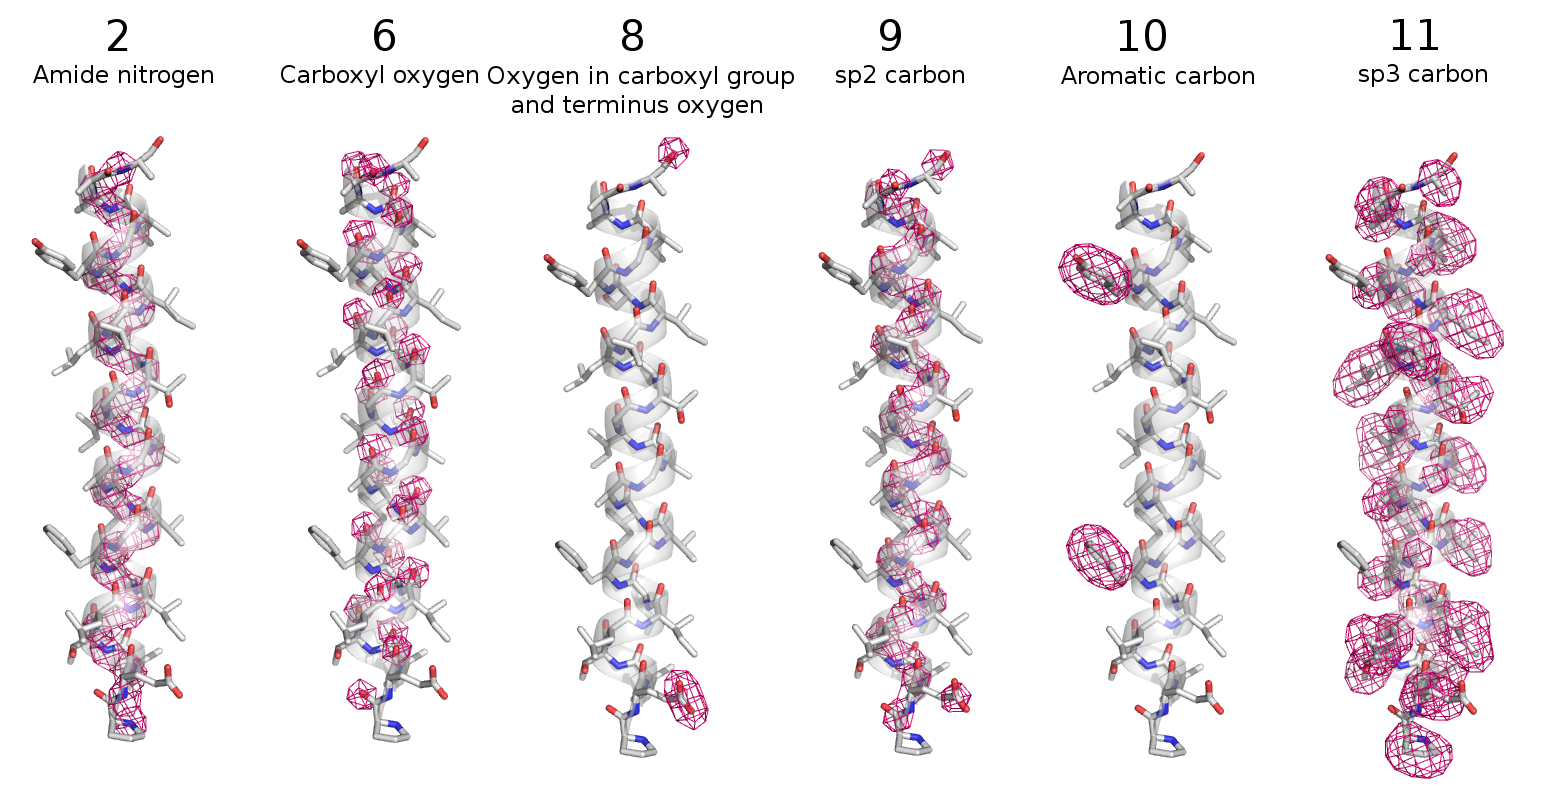
\includegraphics[width=\linewidth]{Fig/atomic_densities_V3.eps}

    \caption{Representation of a protein structure (PDB code 5eh6)
    using atomic densities. The density maps are calculated according
    to Eq.~\ref{eq:rho} and rendered using Pymol \cite{PyMOL} with an
    isosurface level of $0.5$.}

    \label{Fig:atomic_densities}
\end{figure}
